\documentclass[]{report}
\usepackage{geometry}
\usepackage[utf8]{inputenc}
\usepackage{amsmath}
\usepackage{amsfonts}
\usepackage{amssymb}
\usepackage[pdftex]{graphicx}
\usepackage[space]{grffile}
\usepackage{epstopdf}
\usepackage{epsfig}
\usepackage{bmpsize}
\graphicspath{{C:/Users/James/Documents/Benutzerhandbuch//}}
\usepackage[export]{adjustbox}
\usepackage{wrapfig}
\usepackage{appendix}
\usepackage{listings}
\usepackage{hyperref}
\hypersetup{
	colorlinks=true,
	allcolors=blue,
	pdfborderstyle={/S/U/W 1}
}
\usepackage{hypcap}

\title{THM Benutzerhandbuch \\Untis \& THM Organizer}
\author{James Antrim}

\begin{document}
\maketitle

\newpage
\thispagestyle{empty}
\section*{}

\newpage
\tableofcontents
\thispagestyle{empty}

\newpage
\setcounter{page}{1}
\chapter{Allgemeine Untis Bedienungshinweise}

Guten Tag! Ich wollte mal ein kleines Handbuch erstellen bezogen auf unsere Datenhaltung und Arbeitsweise hier an der THM. Alle Angaben beziehen sich auf Untis Version 2014. Ich hatte nicht die Zeit dieses Handbuch, zur Korrektur zu geben. Bitte Verzeihen Sie die vielen Rechtschreib-Fehler.



\section{Felder der Ansicht}

\begin{wrapfigure}{r}{0.4\textwidth}
	\vspace{-15pt}
	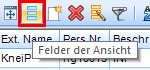
\includegraphics[width=.38\textwidth]{FelderDerAnsicht}
	\vspace{-5pt}
	\caption{Felder der Ansicht Icon}
	\label{fig:fda1}
\end{wrapfigure}
Untis von sich aus setzt eine 'korrekte' Datenpflege nur teilweise voraus. Es stellt für jede Ressource und Unterricht ein Standardsatz an Felder, die ausgefüllt werden dürfen. Jedoch muss man Ressourcen nur einen Namen geben und Unterrichte eine Anzahl an Stunden um diese anzulegen. Bei Unterrichten wird sogar die Zahl eins eingepflegt sofern irgendeine andere Angabe eingepflegt wurde.\\
\\
Damit wir möglichst aussagekräftige Daten haben im System, müssen oft Felder erst eingeblendet werden. Diese werden über die Schnittstelle ``Felder der Ansicht" eingeblendet. Um zu dieser Schnittstelle zu gelangen sucht man in der Ressourcen- oder Unterrichtstoolbarleiste nach drei übereinander gestapelte blaue Rechtecke, wie in Figure \ref{fig:fda1}.

\newpage
\begin{wrapfigure}{r}{0.4\textwidth}
	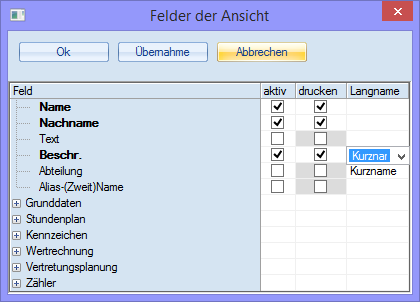
\includegraphics[width=.38\textwidth,right]{FelderDerAnsicht2}
	\vspace{-15pt}
	\caption{Felder der Ansicht}
	\label{fig:fda2}
\end{wrapfigure}

\noindent
Von dieser Schnittstelle aus kann man Häkchen setzen bei den Felder, die man eingeblendet haben oder vom Ansicht entfernen möchte, setzen bzw. entfernen.  Hier kann man auch auswählen wie die entsprechende Angaben anzuzeigen sind. Kurzname zeigt nur der Inhalt des Felds Name der jeweiligen Ressource an. Langname zeigt der Inhalt der Langname, bzw. Nachname, Feld an und Kurzname + Langname zeigt der Inhalt der Name und Langname, bzw. Nachname, Feldes getrennt durch einen ``/" an.\\
\\
Die Anzeige des Langnamens kann von großen Vorteil für das Verständnis der Angaben sein, besonders bei Fächer mit kryptischen Kurznamen. Dennoch ist diese Hilfe mit Vorsicht zu genießen, denn der Ausgabe als Langname allein verleiht man das Gefühl, dass man auch die Langnamen bei der Eingabe verwenden könnte.

\section{Filter}

\section{Sortierung}

\section{Font Einstellungen}

\begin{wrapfigure}{r}{0.4\textwidth}
	\vspace{-15pt}
	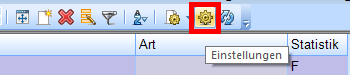
\includegraphics[width=.38\textwidth,right]{Font}
	\vspace{-15pt}
	\caption{Einstellungen (Font) Icon}
	\label{fig:font}
	\vspace{15pt}
	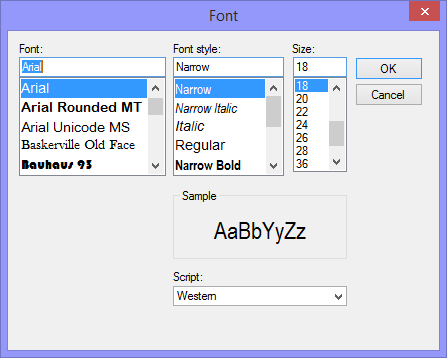
\includegraphics[width=.38\textwidth,right]{Font2}
	\vspace{-15pt}
	\caption{Font Auswahl Ansicht}
	\label{fig:font2}
\end{wrapfigure}

Die Standard Schriftart in Untis ist Arial 8. Diese kann man bei Ressourcen über die Font Ansicht die man kurioserweise über ``Einstellungen", ein gelbes Zahnrad in der Ressourcentoolbarleiste, ändern.\\
\\
Die Ansicht lässt einen den Font, Stil und Größe aussuchen. Mittig im Ansicht gibt es einen kleinen Vorschau wie die ausgewählten Angaben die Ausgabe beeinflussen würden. Mit einem Klick auf dem ``OK" Knopf werden die Änderungen in der jeweilige Ansicht sichtbar.\\
\\
Bei der Erstellung des Lehrplan ruft der ``Einstellungen" Knopf tatsächlich eine Einstellungen Ansicht auf. Bisher ist mir einen Weg den Font des Lehrplans zu ändern nicht bekannt.

\chapter{Datenpflege in Untis}

\begin{wrapfigure}{r}{0.4\textwidth}
	\vspace{-15pt}
	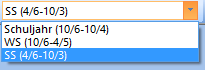
\includegraphics[width=.38\textwidth,right]{Perioden}
	\vspace{-15pt}
	\caption{Perioden}
	\label{fig:mf-sg}
\end{wrapfigure}

\section{Allgemeine Hinweise zur Datenpflege}
Der Semester ist in der Regel der Hauptplanungsabschnitt an der THM. Diese werden mit sogenannten "Perioden" in Untis modelliert. Diese Einheiten sind bereits eingepflegt. Man kann zwischen den jeweiligen Perioden mittels eine Auswahlbox in der obere Menüleiste.\\
\\
Die Perioden werden hier erwähnt, weil \textbf{die Pflege von Gruppen, Räume und Dozenten unbedingt in der Periode ``Schuljahr" gemacht werden sollte}. Wenn Daten in der Schuljahr Periode eingepflegt sind, werden die neuen Daten, bzw. Änderungen, automatisch im Winter- und Sommersemester Perioden ersichtlich. Sollte aber neue Stammdaten oder Änderungen auf bestehenden Stammdaten in die Winter- oder Sommersemester Perioden durchgeführt werden, sind diese Daten nur in diese eine Periode ersichtlich.\\
\\
Bei einzelne Datensätze ist \textbf{Name} ist ein Schlüsselwert, der das schnelle eintippen diese Ressource in Untis ermöglicht. Er soll dementsprechend so kurz und aussagekräftig wie möglich, gehalten werden. Der \textbf{Langname} hingegen enthält den tatsächlichen Namen der jeweilige Ressource. \textbf{Ext. Name} ist ein Fachbereich-übergreifender Name. Er ermöglicht die Sicht auf die Planung der Ressource außerhalb des eigenen Fachbereiches.\\
\\
Die Angabe der \textbf{Name} und \textbf{Langname} ist immer \textbf{Pflicht}.

\newpage
\section{Studiengänge (Abteilungen)}

\begin{wrapfigure}{r}{0.4\textwidth}
	\vspace{-14pt}
	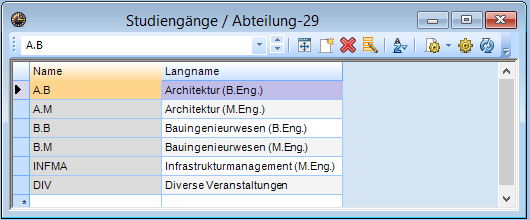
\includegraphics[width=.38\textwidth]{Programs}
	\vspace{-5pt}
	\caption{Studiengänge}
	\label{fig:programs}
	\vspace{24pt}
	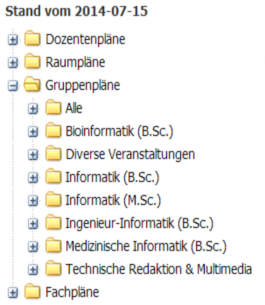
\includegraphics[width=.38\textwidth]{ProgramNavigation}
	\vspace{-5pt}
	\caption{Studiengang Navigation}
	\label{fig:program-navigation}
	\vspace{24pt}
	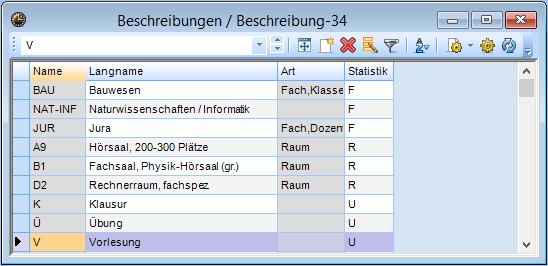
\includegraphics[width=.38\textwidth,right]{Descriptions}
	\vspace{-15pt}
	\caption{Beschreibungen}
	\label{fig:descriptions}
	\vspace{-45pt}
\end{wrapfigure}

Studiengänge erreicht man in dem man in der obere Menüleiste ``Stammdaten" $\triangleright$ ``Spezielle Daten" $\triangleright$ ``Studiengänge" (bzw. ``Abteilungen") auswählt.\\
\\
\textbf{Name}: Die typische Schreibweise besteht aus ein paar Buchstaben die der Name andeuten. Im Falle Zweideutigkeit (Bachelor vs. Master),wird typischerweise die erste Buchstabe der Abschluss nach einem Punkt angehängt.\\

\noindent
\textbf{Langname}: Der Namen des Studiengangs mit abgekürztem Abschluss in runden Klammern dahinter. Dieser Wert wird öffentlich verwendet in der Navigation eines Stundenplans in THM Organizer.

\section{Beschreibungen}

Beschreibungen sind eine Untis-Ressource, die von mehreren weiteren Ressourcen verwendet wird. An der THM wird diese Ressource für Kompetenzen, Raumkategorien und Unterrichtsmethoden. In Untis und THM Organizer werden die Unterrichtsmethoden in der Darstellung benutzt um genau diese Informationen preis zu geben.\\
\\
Sie erreicht man in dem man in der obere Menüleiste ``Stammdaten" $\triangleright$ ``Spezielle Daten" $\triangleright$ ``Beschreibungen" auswählt. Hier ist die Schreibweise der einzelne Felder nach Verwendungszweck unterschiedlich.\\
\\
\textbf{Art}: wird automatisch von Untis gefühlt sofern der Eintrag bereits verwendet wird. Sprich man kann nicht im voraus die Verwendungszweck definieren. (\textbf{Nur indirekt zu beeinflussen})\\
\\
\textbf{Statistik}: wird von uns verwendet um die tatsächliche Verwendung festzulegen. (\textbf{Pflicht})

\newpage
\subsection{Kompetenzen}
\label{subsec:kompetenzen}

\begin{wrapfigure}{r}{0.4\textwidth}
	\vspace{-15pt}
	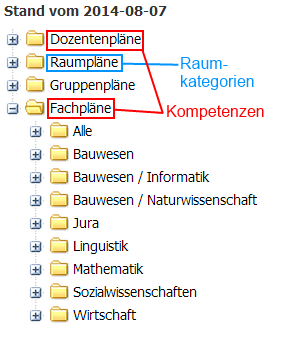
\includegraphics[width=.38\textwidth,right]{DescNavigation}
	\vspace{-25pt}
	\caption{Beschreibungen Navigation}
	\label{fig:description-navigation}
\end{wrapfigure}

Kompetenzen sagen was aus über den groben Inhalt von Gruppen und Fächer, oder die Themengebiete in der sich ein Dozent ein Experte ist.\\
\\
Derzeit sind die \textbf{Namen} und \textbf{Langnamen} nach einem von Herr Kneisel entworfenes System aufgebaut. Dieses System besteht aus Basis-Kompetenzen, die jeweils durch drei Buchstaben gekennzeichnet sind. Diese entsprechen ein recht grobes Themengebiet wie Naturwissenschaft oder Bauingenieurwesen. Zusätzlich gibt es die Möglichkeit Hybride-Kompetenzen zu erschaffen. Die Namen von Hybride-Kompetenzen werden durch die Bezeichner von zwei Basis-Kompetenzen verbunden durch einem Minus-Zeichen gekennzeichnet. Ihre \textbf{Langnamen} entsprechend durch die Langnamen zweier Basis-Kompetenzen getrennt durch `` / ". In der \textbf{Statistik}-Spalte kommt die Buchstabe ``F" (für Fachkompetenz).\\
\\
Hier wäre eine Überarbeitung des Systems grundsätzlich erwünschenswert. Beispielsweise Fachbereich Wirtschaft hat, zusätzlich zu den Einträgen vom Kneisel-System, neun Schwerpunkte, wie Mittelstand oder Marketing. Diese Schwerpunkte sind um einiges aussagekräftiger und relevanter für Studenten und Dozenten.

\subsection{Raumkategorien}
\label{subsec:roomcategory}

Raumkategorien sagen was aus über der Raumtyp und machen Andeutungen auf dessen Kapazität oder Ausstattung.\\
\\
Der \textbf{Name} und der \textbf{Langname} von Raumkategorien beziehen sich auf einem System entwickelt von Herr Deniffel für die THM. Der \textbf{Name} besteht meist aus einer Buchstabe und einer Zahl. ``A" zum Beispiel, bedeutet Seminarraum oder Hörsaal, wohingegen ``D" ein Rechnerraum kennzeichnet. Die Zahlen beziehen sich auf Raumeigenschaften wie Größe oder Ausstattung. Bei A2 heißt das ``2" 21 bis 33 Sitzplätze, bei D2 hingegen heißt die ``2", dass in dem Raum eine fachspezifische Ausstattung sich befindet. Der \textbf{Langname} ist eine von Kommata getrennte Auflösung dieser zwei Teile. Hier wird ein ``R" (für Raumkategoire) im \textbf{Statistik} Feld eingetragen.\\
\\
Eine vollständige Liste der Raumkategorien befindet sich im Dennifelsche Raumkategorien \ref{sec:dennifel}.

\newpage
\subsection{Unterrichtsmethoden}

Unterrichtsmethoden beschreiben der Form der Instanzen eines Unterrichts.\\
\\
Der \textbf{Name} besteht meist aus einer Buchstabe, wie ``V" für Vorlesung oder ``L" für Labor. Der \textbf{Langname} entsprechend der ausführliche Schreibweise. Sollte ein Unterrichtsinstanz mehrere Methoden verwenden sollen, können auch hier Hybride-Methoden erschaffen. Hier werden die einfachen Angaben durch ein ``/" getrennt, wie ``V/Ü" (Vorlesung/Übung) oder ``V/P" (Vorlesung/Praktikum). Für Unterrichtsmethoden ist die entsprechende \textbf{Statistik} ``U".\\
\\
In THM Organizer werden diese Angaben als Teil des Unterrichtsnamens ausgegeben.

\begin{figure}[htbp]
	\begin{minipage}{0.5\linewidth} 
		\centering
		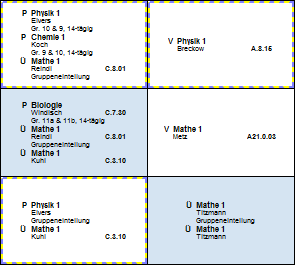
\includegraphics[width=.45\textwidth]{MethodsUntis}
		\vspace{-5pt}
		\caption{Unterrichtsmethoden Untis}
		\label{fig:methoden-untis}
	\end{minipage}
	\begin{minipage}{0.5\linewidth}
		\centering
		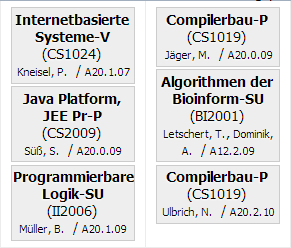
\includegraphics[width=.45\textwidth]{MethodsOrganizer}
		\caption{Unt.meth. THM Organizer}
		\label{fig:methoden-organizer}
	\end{minipage}
\end{figure}

\newpage
\section{Gruppen (Klassen)}

Gruppen, auch Klassen in Untis genannt, sind zugleich Zielgruppe und Angebot für eine Menge an Unterrichten, und werden nach das eine oder das andere genannt. Zum Beispiel eine Gruppe mit der Name ``1. Semester" oder ``Schwerpunkt Wirtschaftsinformatik" bezeichnet sowohl die Gruppe von Studenten die eine Gruppe von Unterrichte besuchen soll, als auch die Menge an Unterrichte die diese Studenten besuchen.\\
\\
Sie erreicht man in dem man in der obere Menüleiste ``Stammdaten" $\triangleright$ ``Gruppen" oder ggf. ``Klassen" auswählt.

\begin{figure}[h]
	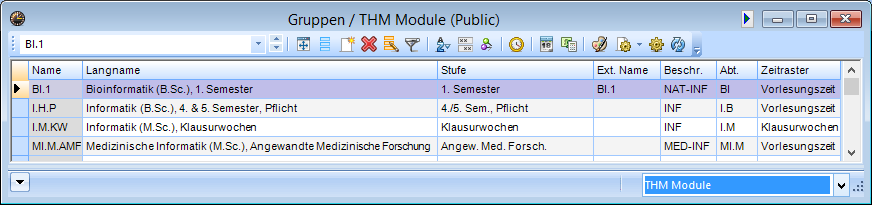
\includegraphics[width=1\textwidth]{Gruppen}
	\vspace{-15pt}
	\caption{Gruppen}
	\label{fig:groups}
\end{figure}

\noindent
\textbf{Name}: Beinhaltet Hinweise auf den jeweiligen Studiengang, sowie die spezifische Untergliederung. Typischerweise mit Punkten getrennt.\\
\\
\textbf{Langame}: Der ausgeschriebene Name des Studiengangs mit Abschluss in runden Klammern, gefolgt von Untergliederungsteile, getrennt durch Kommas.\\
\\
\textbf{Ext. Name}: (\textbf{Pflicht bei Fachbereichübergreifende Studiengänge, sonst Optional})\\
\\
\begin{wrapfigure}{r}{0.4\textwidth}
	\vspace{-10pt}
	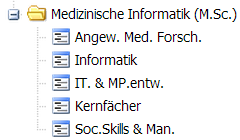
\includegraphics[width=.38\textwidth]{MedInfNodes}
	\vspace{-5pt}
	\caption{Stufen (Med. Inf. Pläne)}
	\label{fig:steps}
\end{wrapfigure}
\textbf{Stufe}: Eine Kurzfassung der Untergliederung. Wird als Plan Name in der Navigation in THM Organizer benutzt.(\textbf{Pflicht})\\
\\
\textbf{Beschr. (Kompetenz)}: Assoziiert die Gruppe mit einer Kompetenz. (Sehe Kompetenzen, Subsection  \ref{subsec:kompetenzen}, \textbf{Pflicht)})\\
\\
\textbf{Abt. (Studiengang)}: Assoziiert die Gruppe (und durch Implikation zugeordnete Unterrichte) mit einem Studiengang. (\textbf{Pflicht})\\
\\
\textbf{Zeitraster}: Assoziiert die Gruppe mit einem Zeitraster. Standardmäßig ist dieser Wert ``Hauptzeitraster". Falls Multi-Zeitraster aktiviert ist kann man eine eingepflegte Zeitraster auswählen. (\textbf{Pflicht, wird automatisch gefüllt})

\subsection{Zeitraster}

Zeitraster legen die Blöcke fest in dem man Unterrichtsinstanzen unterbringen kann. An der THM haben wir bisher zwei feste Zeitraster, eine für Vorlesungen und eine für die Klausurwochen. Sprich, unsere Zeitraster sind an Festen Daten gebunden.\\
\\
Untis, jedoch, bindet diese Ressource an Klassen. Wo Zeitraster für uns eine Antwort auf die Frage ``wann" sind, sind sie in Untis eine Antwort auf die Frage ``was" oder ``für wen". Dies bewirkt das wir ein wenig umdenken müssen um die Klausurwochen modellieren zu können. Mehr dazu in der nächsten Version dieses Handbuchs.

\newpage
\section{Dozenten (Lehrer)}

Dozenten bezeichnen Festangestellte Dozenten, Lehrbeauftragte, Tutoren und Vortragende.\\
\\
Sie erreicht man in dem man in der obere Menüleiste ``Stammdaten" $\triangleright$ ``Dozenten" oder ggf. ``Lehrer" auswählt.

\begin{figure}[h]
	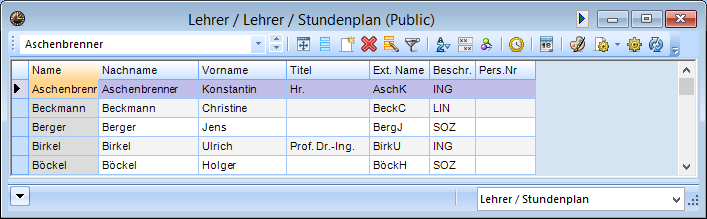
\includegraphics[width=1\textwidth]{Teachers}
	\vspace{-15pt}
	\caption{Dozenten}
	\label{fig:teachers}
\end{figure}

\noindent
\textbf{Name}: Typischerweise bestehend aus die Nachnamen. Sollten mehrere Dozenten der gleiche Nachname haben, werden Buchstaben der Vorname zwecks Eindeutigkeit angehängt. \\
\\
\textbf{Nachname}: Die Nachnamen des Dozenten.\\
\\
\begin{wrapfigure}{r}{0.4\textwidth}
	\vspace{-10pt}
	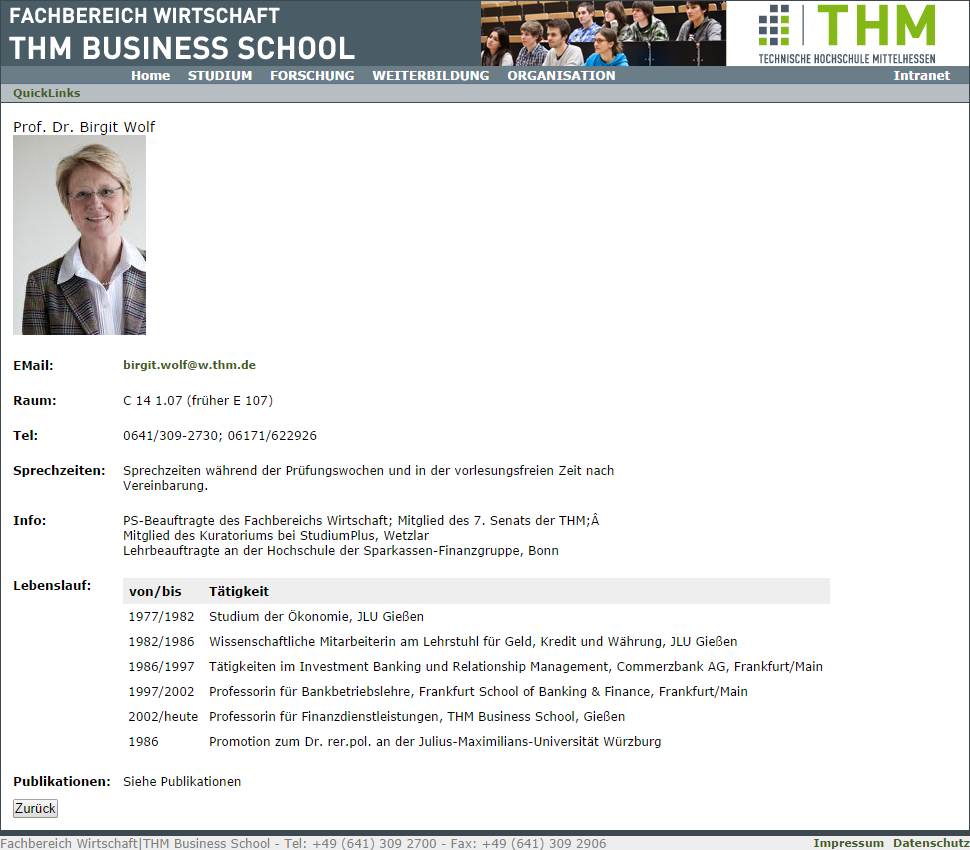
\includegraphics[width=.38\textwidth]{GroupsProfile}
	\vspace{-5pt}
	\caption{THM Groups Profile}
	\label{fig:thmgroupsprofile}
\end{wrapfigure}
\textbf{Vorname}: Die Vornamen des Dozenten.(\textbf{Empfohlen})\\
\\
\textbf{Titel}: Der Titel des Dozenten.(\textbf{Optional})\\
\\
\textbf{Ext.Name}: (\textbf{Pflicht, falls gewünschter Dozent nicht vorhanden bitte an mich wenden})\\
\\
\textbf{Beschr.(Kompetenz)}: Assoziiert der Dozent mit einem Kompetenz. (Sehe Kompetenzen, Subsection  \ref{subsec:kompetenzen}, \textbf{Pflicht)})\\
\\
\textbf{Pers.Nr(THM Benutzerkennung)}: Die THM Benutzerkennung des Dozents. Ermöglicht ggf. die Verlinkung auf einem THM Groups Benutzer-Profile aus THM Organizer. (\textbf{Optional})\\

\newpage
\section{Räume}

Räume bezeichnen sämtliche Orte wo Unterrichte, Vorträge, Sitzungen und sonstige Stundenplan relevante Ereignisse stattfinden. Obwohl stereotypische Räume wie Hörsäle, Besprechungsräume, Labore machen den Großteil der Raumbestand aus, auch außergewöhnliche Ortschaften wie der Grillplatz, Kongresshalle, Krankenhäuser, oder gar ``Online" sind auch vertreten.\\
\\
Sie erreicht man in dem man in der obere Menüleiste ``Stammdaten" $\triangleright$ ``Räume" auswählt.

\begin{figure}[h]
	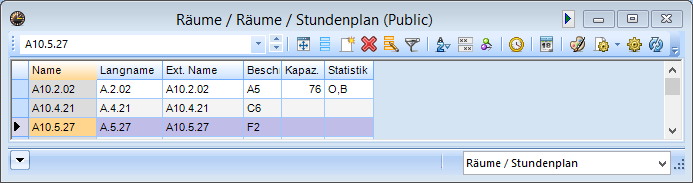
\includegraphics[width=1\textwidth]{Rooms}
	\vspace{-15pt}
	\caption{Räume}
	\label{fig:rooms}
\end{figure}

\noindent
\textbf{Name}: Weil die Namen eindeutig sein müssen, werden Räume die mit A und C anfangen mit A10 bzw. C10 versehen.\\
\\
\textbf{Langname}: Die aktuelle Bezeichnung für den Raum.\\
\\
\textbf{Ext.Name}: Das Selbe wie der \textbf{Name}. (\textbf{Pflicht})\\
\\
\textbf{Beschreibung}: Das Selbe wie der \textbf{Name}. (Sehe Raumkategorien, Subsection  \ref{subsec:roomcategory}, \textbf{Pflicht)})\\
\\
\textbf{Kapaz.(Kapazität)}: Die Anzahl der Sitzplätze für Studenten. (\textbf{Optional})\\
\\
\textbf{Statistik(Ausstattung)}: Einstellige Bezeichner für die Ausstattung des Raums, wie Overhead (O), Beamer (B). Die Bezeichner werden durch Kommate getrennt. Diese werden von Untis eingefügt, der Benutzer braucht sich nicht darum zu kümmern. (\textbf{Optional})\\

\newpage
\subsection{Raumgruppen}

Raumgruppen sind Gruppierungen von Räumen nach Typ, Ausstattung, Kapazität, Verwendungszweck, eine Kombination daraus, oder was man sonst noch einfällt. In Figure \ref{fig:roomgroups} sieht man drei der Gruppen die Fachbereich MNI verwendet. Die erst Gruppe, LPC, beinhaltet eine Auflistung der Rechnerlabore in Gebäude A20, jeweils von gleichen Typ, mit einer ähnlichen Ausstattung und Kapazität.\\
\\
Raumgruppen an sich sind \textbf{optional}. Sie sind lediglich eine Hilfestellung zur Raumsuche. Sie werden in der Lehrplanung eingetragen und, sofern die zugewiesene Räume nicht erschöpft sind, muss man erst gar nicht nach einem geeigneten Raum suchen. Mehr Dazu später in Rooms, Subsection \ref{subsec:rooms}, von Lehrplanung (\ref{sec:lehrplanung}).\\
\\ 
Sie erreicht man in dem man in der obere Menüleiste ``Stammdaten" $\triangleright$ ``Spezielle Daten" $\triangleright$ ``Raumgruppen" auswählt.

\begin{figure}[h]
	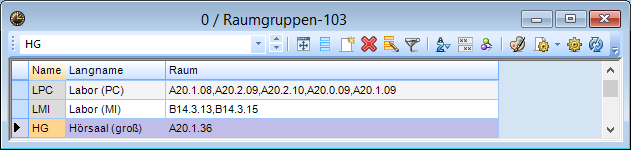
\includegraphics[width=1\textwidth]{RoomGroups}
	\vspace{-15pt}
	\caption{Raumgruppen}
	\label{fig:roomgroups}
\end{figure}

\noindent
\textbf{Name}: (\textbf{Pflicht, sofern verwendet})\\
\\
\textbf{Langname}: (\textbf{Optional, die Langnamen werden nicht verwendet})\\
\\
\textbf{Raum}: Eine, durch Kommata getrennte, Liste der Räume, die dieser Gruppe zugehören sollen. Hier gibt es keine Eingabehilfe seitens Untis.(\textbf{Pflicht, sofern verwendet})\\

\newpage
\section{Fächer}

Fächer sind die Namensträger für die Unterrichte und Unterrichtsinstanzen. Sie geben einen Hinweis darauf, welche Lerninhalte in einem Unterricht oder Unterrichtsinstanz übermittelt werden. Der Begriff Fach bezeichnet hier auch die mehr-fachigen Module sofern diese der gewünschte Name für die Ausgabe ist.\\
\\
Zum Beispiel besteht das Modul International Marketing im Studiengang Unternehmensführung aus mehrere Fächer, im Stundenplan ist nur einer Name für alle solche Fächer gewollt. Im Gegensatz dazu stehen Module wie Theorie des Entwerfens I aus Studiengang Bauingenieurwesen, hier sind die Namen der untergeordneten Fächer Einführung ins Entwerfen und Baugeschichte der Ausgabe gewollt und müssen deshalb getrennt eingepflegt werden.\\
\\ 
Fächer haben die besondere Eigenschaft, dass allein Sie müssen nicht im Schuljahr-Periode gepflegt werden, sondern jegliche Änderungen an einem Fach sind sofort in allen Perioden sichtbar. Sie erreicht man in dem man in der obere Menüleiste ``Stammdaten" $\triangleright$ ``Fächer" auswählt.

\begin{figure}[h]
	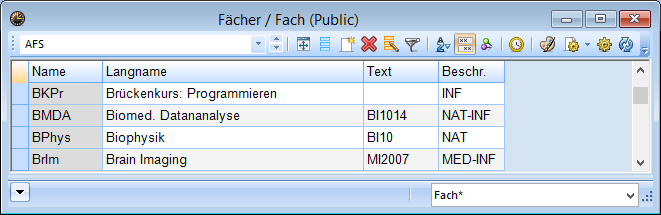
\includegraphics[width=1\textwidth]{Subjects}
	\vspace{-15pt}
	\caption{Fächer}
	\label{fig:subjects}
\end{figure}

\noindent
\textbf{Name}: (\textbf{Pflicht})\\
\\
\textbf{Langame}: (\textbf{Pflicht})\\
\\
\textbf{Text(Modulnummer)}: Die Modulnummer des Faches. Hier ist entscheidend, wie die Modulen in LSF abgelegt werden, denn diese Angabe verhilft die Weiterleitung auf Modulbeschreibungen. Sollten Module nicht atomar gehalten werden, weißt man nicht unbedingt ob die Beschreibungen auf der Ebene der Module oder auf Ebene des Faches liegen. Im Zweifelsfall pflegen wir diese Angaben gemeinsam.(\textbf{Empfohlen})\\
\\
\textbf{Beschr.(Kompetenz)}: Assoziiert das Fach mit einem Kompetenz. (Sehe Kompetenzen, Subsection  \ref{subsec:kompetenzen}, \textbf{Pflicht)})

\newpage
\section{Unterrichtsgruppen}

Unterrichtsgruppen sind grobe Rahmen für dien Daten an den Veranstaltungen stattfinden. Ohne der Angabe der Unterrichtsgruppe haben Unterrichte standardmäßig einen Lauf über das gesamte Semester einschließlich Projektwochen, Klausurwochen, usw.\\
\\


\chapter{Unterrichtplanung}

Die Unterrichtsplanung in Untis geschieht in zwei Schritte die Lehrplanung in der abstrakte Unterrichte eingepflegt werden und die Stundenplanung in der die Instanzen mit einer festen Zeit und Raum verbunden werden.

\section{Lehrplanung}
\label{sec:lehrplanung}


\subsection{Räume}
\label{subsec:rooms}

\section{Stundenplanung}

\begin{appendices}
\chapter{Zusatzmaterial}
\section{Dennifelsche Raumkategorien}
\label{sec:dennifel}

\begin{description}
	\item[A1] Seminarraum, 1-20 Plätze
	\item[A2] Seminarraum, 21-33 Plätze
	\item[A3] Seminarraum, 34-47 Plätze
	\item[A4]	Hörsaal,  48- 69 Plätze
	\item[A5]	Hörsaal,  70- 84 Plätze
	\item[A6]	Hörsaal,  85-105 Plätze
	\item[A7]	Hörsaal, 100-150 Plätze
	\item[A8]	Hörsaal, 150-200 Plätze
	\item[A9]	Hörsaal, 200-300 Plätze
	\item[AZ]	Hörsaal, 300-400 Plätze
	\item[B1]	Fachsaal, Physik-Hörsaal (gr.)
	\item[B2]	Fachsaal, Physik-Hörsaal (kl.)
	\item[B3]	Fachsaal, Chemie	Raum	R
	\item[C1]	Fachsaal, Praktikumsraum mit. spez. Einbauten
	\item[C2]	Fachsaal, Praktikumsraum keine spez. Einbauten
	\item[C3]	Fachsaal, Forschungslabor
	\item[C4]	Fachsaal, Mess-Stand
	\item[C5]	Fachsaal, Nebenlabor
	\item[C6]	Fachsaal, Vorbereitungsraum
	\item[C9]	Fachsaal, Betriebsraum
	\item[D1]	Rechnerraum, allgemein
	\item[D2]	Rechnerraum, fachspez.
	\item[D3]	Rechnerraum, fachspez. (Forschung)
	\item[D4]	Rechnerraum, Peripherie- / Geräteraum
	\item[D5]	Rechnerraum, Serverraum
	\item[D7]	Rechnerraum, Schulung
	\item[F1]	Projektraum, allgemein
	\item[F2]	Projektraum, Gruppenarbeitsraum
	\item[F3]	Projektraum, Übungen
	\item[F5]	Projektraum, Studiebüro
	\item[F6]	Projektraum, Sozialraum
	\item[H1]	Sonstige Räume, Archiv
	\item[H2]	Sonstige Räume, Seminar-Nebenraum
	\item[H3]	Sonstige Räume, sonstiges Lager
	\item[H4]	Sonstige Räume, Labor Lager
	\item[H5]	Sonstige Räume, Abstellraum
	\item[I1]	Büro, Büro	Raum
	\item[I2]	Büro, Labor-Ingenieur
	\item[I3]	Büro, Werkstatt
	\item[I4]	Büro, Besprechungen
	\item[I5]	Büro, Ergänzungsraum
	\item[I6]	Büro, Videokonferenzen
	\item[UNIMA]	Raum, Uni Marburg
	\item[W1]	Werkstatt, Feinmechanik
	\item[W2]	Werkstatt, Metall
	\item[W5]	Werkstatt, Elektronik
	\item[W7]	Werkstatt, Nebenraum
	\item[W9]	Werkstatt, Lager
	\item[X]	Raum, nicht bekannt
\end{description}

\section{Unterrichtsgruppen 2014/2015}
\label{sec:unterrichtsgruppen-values}
\begin{description}
	\item[WS.E]	Einführungswoche - WS 06.10.2014 - 11.10.2014	 	 	 	
	\item[WS]	Wintersemester	13.10.2014 - 31.01.2015	
	\item[WS.A]	Wintersemester (Woche A) 13.10.2014 - 31.01.2015
		\begin{itemize}
			\item 13.10.2014 - 18.20.2014
			\item 27.10.2014 - 01.11.2014
			\item 10.11.2014 - 15.11.2014
			\item 24.11.2014 - 29.11.2014
			\item 08.12.2014 - 13.12.2014
			\item 12.01.2015 - 17.01.2015
			\item 26.01.2015 - 31.01.2015
		\end{itemize}
	\item[WS.B]	Wintersemester (Woche B) 20.10.2014 - 24.01.2015
		\begin{itemize}
			\item 20.10.2014 - 25.10.2014
			\item 03.11.2014 - 08.11.2014
			\item 17.11.2014 - 22.11.2014
			\item 01.12.2014 - 06.12.2014
			\item 15.12.2014 - 20.12.2014
			\item 19.01.2015 - 24.01.2015
		\end{itemize}
	\item[WS.P]	Projektwoche - WS 05.01.2015 - 10.01.2015	 	 	 	
	\item[WS.K1] Klausurwoche 1 - WS	2/2/2015	2/8/2015	 	 	 	
	\item[WS.K2] Klausurwoche 2 - WS	2/9/2015	2/15/2015	 	 	 	
	\item[WS.B1] Blockveranstaltungen 1 - WS	2/16/2015	3/1/2015	 	 	 	
	\item[WS.B2] Blockveranstaltungen 2 - WS	3/2/2015	3/15/2015	 	 	 	
	\item[WS.K3] Klausurwoche 3 - WS	3/23/2015	3/29/2015	 	 	 	
	\item[WS.K4] Klausurwoche 4 - WS	3/30/2015	4/5/2015	 	 	 	
	\item[SS.E]	Einführungswoche - SS	4/6/2015	4/12/2015	 	 	 	
	\item[SS] Sommersemester	4/13/2015	7/19/2015  6/1	6/7
	\item[SS.A] Sommersemester (Woche A)	4/13/2015	7/19/2015 4/20	4/26
		SS.A	Sommersemester (Woche A)	4/13/2015	7/19/2015 5/4	5/10
		SS.A	Sommersemester (Woche A)	4/13/2015	7/19/2015 5/18	5/24
		SS.A	Sommersemester (Woche A)	4/13/2015	7/19/2015 6/1	6/14
		SS.A	Sommersemester (Woche A)	4/13/2015	7/19/2015 6/22	6/28
		SS.A	Sommersemester (Woche A)	4/13/2015	7/19/2015 7/6	7/12
	\item[SS.B]	Sommersemester (Woche B)	4/20/2015	7/12/2015 4/27	5/3
		SS.B	Sommersemester (Woche B)	4/20/2015	7/12/2015 5/11	5/17
		SS.B	Sommersemester (Woche B)	4/20/2015	7/12/2015 5/25	6/7
		SS.B	Sommersemester (Woche B)	4/20/2015	7/12/2015 6/15	6/21
		SS.B	Sommersemester (Woche B)	4/20/2015	7/12/2015 6/29	7/5
	\item[SS.P]	Projektwoche - SS	6/1/2015	6/7/2015	 	 	 	
	\item[SS.K1]	Klausurwoche 1 - SS	7/20/2015	7/26/2015	 	 	 	
	\item[SS.K2]	Klausurwoche 2 - SS	7/27/2015	8/2/2015	 	 	 	
	\item[SS.B1]	Blockveranstaltungen 1 - SS	8/3/2015	8/16/2015
	\item[SS.B2]	Blockveranstaltungen 2 - SS	8/17/2015	8/30/2015
	\item[SS.K3]	Klausurwoche 3 - SS	9/21/2015	9/27/2015	 	 	 	
	\item[SS.B3]	Blockveranstaltungen 3 - SS	9/7/2015	9/20/2015
	\item[SS.K4]	Klausurwoche 4 - SS	9/28/2015	10/4/2015 	 	 	
		
\end{description}

	
\end{appendices}

\end{document}          
